% *TODO*
% say more clearly there are 3 methods for approximation so far: LP & region growing; LP & distance
% pivot; combinatorial pivot
% say that in practice, general graphs are assumed to be complete with missing edges being negative
% - “The problem is agnostic in the sense that the clustering of the data is not taken into account
%   or even assumed to exist.” another way to look at it is that we're trying to get a binary
%   classifier of edges (+ or -) using an hypothesis class (nodes clustering) with limited
%   expression power (as it has to respect transitivity constraints, whereas signs can be inconsistent)
% - when the graph is weighted, there is no much point separating complete from
%   general since weights can be 0

As mentioned earlier, most real signed graphs are not fully balanced and thus do not have a
perfectly consistent clustering. The problem of quantifying how much a given graph departs from this
ideal situation is called \pcc{}. After defining it formally in \autoref{sub:problem_setting}, we
show that \pcc{} is a learning problem on its own, and discuss how it relates to the binary
classification problem of predicting edge signs, among many others applications. We then present
numerous methods to solve \pcc{} in \autoref{sub:state_of_the_art}, ranging from exact methods (that
implicitly leverage our bias) to heuristics (whose greedy and energy minimization frameworks are
classic in unsupervised graph cut problems). We also devote a large section to approximation
methods, in order to get a sense of why the problem is \NPc{}. This allows us to finish in
\autoref{sub:cc_non_worst_case} by describing situations related to our bias where is possible to
solve the problem efficiently and optimally. By doing so, we update existing surveys on the same
topic~\autocites{bonchi2014correlation}{surveyCC16}{CCWirth2017}, highlighting the importance of
\pcc{} to solve our binary learning problem.

% surveyCC16 is about mind on complete graph (ie cluster editing). They give a Russian article from
% 1971 that says it cluster editing on triangle-free graph can be solved in polynomial time, which
% include bipartite graph (so for CC, if G^+ is (complete? I think so) bipartite)
% Fridman, G.Š.: A graph approximation problem. Upravlyaemye Sistemy 8, 73–75 (1971). (in Russian)
% In [14] it was observed that the problem is polynomially solvable for instances of at most 2
% clusters??! Actually it means consensus clustering can be solved in polynomial time when there are
% only 2 clustering as input

\subsection{Problem setting and connection to \esp{}}
\label{sub:problem_setting}
Like other clustering frameworks, in \pcc{}, we are given a set of objects and we want to gather
them into groups (called clusters) so that objects belonging to one cluster are similar to each
other while being dissimilar to objects from all the other clusters.

In \pcc{}, we formalize this problem by considering objects as the nodes of a graph $G$, whose edge
weights encode similarity. Namely, in the most general case, for nodes $u$ and $v$, the edge between
$u$ and $v$ is associated with two positive numbers:
$w_{u,v}^+$ denotes the strength of the similarity between $u$ and $v$;
$w_{u,v}^-$ denotes the strength of the dissimilarity between $u$ and $v$.
Note, however, that in many applications, only one of these two numbers is nonzero, in which case
we more conveniently set $w_{u,v} = \begin{cases}
	 w_{u,v}^+ & \quad \text{if } w_{u,v}^+ > 0 \text{ and } w_{u,v}^-=0 \\
	-w_{u,v}^- & \quad \text{if } w_{u,v}^+ = 0 \text{ and } w_{u,v}^->0 \\
\end{cases}$

Now consider a clustering \cluster{} of $V$, that is a function from $V$ to $\Nbb{}^{|V|}_{>0}$
that assigns to each node a cluster index.\marginpars{We will also abuse the notation and let
\cluster{} be a set of clusters $\cluster=\{C_1, C_2, \ldots, C_k\}$ that form a partition of $V$.
That is, $\forall i\,C_i\subset V$, $\bigcup_{i=1}^k C_i = V$ and $\forall i\neq j,\, C_i\cup C_j =
\emptyset$.} For instance, $\cluster(u) = 3$ means that $u$ belongs
to the third cluster. We can evaluate how \cluster{} fits our clustering paradigm in two ways,
either by the number of \emph{agreements}, that is the weighted number of positive edges inside
clusters plus the weighted number of negative edges across clusters; or by the number of
\emph{disagreements}, that is the weighted number of negative edges inside clusters plus the
weighted number of positive edges across clusters. Given a cost function $c$, which is usually the
identity, \pcc{} can then be seen as a graph optimization problem, either of maximizing agreements
(\maxa{}):
\begin{equation}
	\max_{\cluster{}} \sum_{\cluster(u) = \cluster(v)} c(w_{uv}^+) +
	\sum_{\cluster(u) \neq \cluster(v)} c(w_{uv}^-)
	\label{eq:maxa}
\end{equation}
or minimizing disagreements (\mind{})\footnote{Note that in the data mining literature, \pcc{} may
refer to another problem. Namely, it is a special case of high-dimensional data clustering, where
features are locally correlated in various ways across different clusters that reside in arbitrarily
oriented subspaces~\autocite{otherCCproblem09}.}:
\begin{equation}
	\min_{\cluster{}} \sum_{\cluster(u) = \cluster(v)} c(w_{uv}^-) +
	\sum_{\cluster(u) \neq \cluster(v)} c(w_{uv}^+)
	\label{eq:mind}
\end{equation}

Although an optimal clustering $\cluster^\star$ achieves the same value on both \eqref{eq:maxa}
and \eqref{eq:mind}, we will see in \autoref{sub:state_of_the_art} that the latter objective is in
some sense \enquote{easier}. Another interesting feature of the \pcc{} problem is that contrary to
other clustering formulations, it does not require us to set the number of clusters $k$ beforehand.
Instead, $k$ emerges as a natural property of the solution. Since clustering is an unsupervised
problem, this is generally handy. However, in some situations, we may have prior knowledge on how
many clusters are the data, or external constraints. This can be handled with parametrized version
of \pcc{}, namely \maxa$[k]$ and \mind$[k]$ where the optimization is over clustering with exactly
$k$ clusters.

In \autoref{fig:cc_objectives}, we show a simple instance of \pcc{} and one of its optimal solution.
\begin{figure}[hbt]
	\centering
	\includegraphics[width=0.63\linewidth]{assets/tikz/cc_objectives_tikz.pdf}
	\caption[Small example of \pcc{}]{A small graph with eight nodes and ten edges. Solid edges
	represent positive edges and dashed edges represent negative edges. A clustering \cluster{}
	is showed with 3 clusters: $\{1, 2, 4\}$, $\{3, 5, 6\}$ and $\{7, 8\}$. \cluster{} incurs two
	disagreements: the negative edge between nodes $1$ and $2$ within the blue cluster, and the
	positive edge $(6,7)$ between the orange and green clusters. Those disagreements are created
	by two cycles with one negative edge and thus cannot be avoided, meaning that \cluster{} is
	optimal. However, it is not the unique solution: for instance, merging the orange and green
	clusters would also yield two disagreements.}
	\label{fig:cc_objectives}
\end{figure}

\subsubsection{Applications}
\label{ssub:cc_applications}

According to \textcite[Section 5]{Demaine2006}, \pcc{} is well suited to several situations:
\begin{itemize}
   \item when the items to be clustered do not belong to a natural metric space (preventing
      approaches such as $k$-means) but we still know for some pairs whether they are similar or
      not.
   \item when we do not know the number of clusters beforehand but we have a similarity measure. In
      that case, we can select a problem-specific similarity threshold and set all edges with a
      similarity larger than the threshold to be positive while the others are set to negative.
   \item when we have a classic clustering problem (that is a set of objects, a distance between
      them and an objective function to minimize) with additional pairwise constraints of the form
      \emph{must-link/cannot-link}. Instead of restraining a clustering algorithm to the space of
      feasible solution, we convert the distances between objects and the constraints into signed
      edges and solve the resulting \pcc{} problem. 
\end{itemize}

In addition to these general considerations, \pcc{} has also been used in several domains:
%TODO turn those items into paragraphs?
\begin{description}
   \item[Computer Vision]
      The ubiquitous task of segmenting an image into homogeneous regions is a prerequisite for many
      further processing, and can be tackled with \pcc{}. For instance, to segment cell in
      microscopy imagery, \textcite{CellSeg14} first use generic image features to classify pixel in
      belonging to region boundaries or not. Then, they extract small scale regions called
      superpixels. After building the adjacency graph of these superpixels, they assigned edge
      weights by averaging the boundary probabilities of the pixels separating adjacent
      superpixels. They also add strong negative constraints between distant superpixels, and lastly
      cluster these superpixels according to the \pcc{} objective to obtain the final segmentation.
      A similar approach was used earlier in~\textcite{Kim2011}, who stress the importance of
      considering such higher order constraints between distant superpixels in order to achieve good
      performance. This was also extended to 3D segmentation~\autocite{VolumeSegmentation12}, where
      additional tuning allows to segment a volume image of a mouse cortex with up to billions
      voxels. \Textcite{Beier2015} segment 2D and 3D images with an energy based formulation of
      \pcc{} and iteratively improve their solution by merging it with another clustering given by a
      proposal generator. By developing another scalable energy based optimization procedure, and
      with the help of few user-provided cues, \textcite{Bagon2011} are able to apply \pcc{}
      directly at the pixel level.
      % one more? https://link.springer.com/chapter/10.1007/978-3-642-33783-3_41
      % 3D mesh segment https://link.springer.com/article/10.1007/s41095-016-0071-3

      Beyond image segmentation, \textcite{Shape3D17} develop a method to extract a network of
      descriptive curves from 3D shapes.  After an initial stage of generating many such
      \emph{flowlines}, they describe in Section 6 a \pcc{} formulation to extract \emph{reliable}
      representative flowlines, using geometric constraints to obtain positive or negative cues that
      two flowlines are from the same reliable representative.

      Finally, in order to track several targets across sequential video frames,
      \textcite{multiTracking15} propose a multistage framework. One step revolves around a matrix
      $A$ that defines the cost of assigning an object tracked in previous frames to an object
      detected in the current frame. This matrix is turned into a symmetric affinity matrix
      $\bar{A}_{sym}$ that can be seen as a signed graph adjacency matrix. \pcc{} is then used to extract clusters
      (called zones), in which local processing is performed. This is beneficial since the
      complexity of these local methods can be adapted to the difficulty of each zone.

   \item[Natural Language Processing] 
      Coreference resolution is the task of finding all expressions that refer to the same entity in
      a text. Like image segmentation, it is a preprocessing step that can later be used in document
      summarization, question answering, and information extraction. \Textcite[Section
      2.3]{graphicalCoreference04} tackle coreference resolution by using an undirected graphical
      model on which performing inference is equivalent to \pcc{}. On small scale instances,
      \textcite{Elsner2009} first obtain an upper bound of the optimal solution by solving a SDP
      relaxation of the problem. They then compare various heuristics and show that best performing
      ones are within few percents of the optimum, provided they are followed by a local search
      step, such as the Best One Element Move~\autocite{Gionis2007}. Further NLP tasks amenable to
      \pcc{} formulation are referenced in their paper. Another possible task would be 
      to cluster words based on distributional embedding vector while adding antonym
      constraints~\autocite{SignedWordRatings}, although the authors of that paper choose to use
      signed spectral clustering.

   \item[Biology]
      Clustering tasks also abounds in Biology.
      A typical input is a similarity matrix between genes expression level in various experimental conditions
      and the goal is to cluster those genes into groups which react similarly. \Textcite[Section
      4]{Ben-Dor99} gives three examples: 112 genes involved in the rat central nervous system, 1246
      genes of the roundworm \emph{C. elegans} and 2000 human genes obtained from 40 tumor and 22
      normal colon samples. \Textcite{Mason2009} analyze a signed co-expression network of genes
      involved in embryonic stem cells to find which genes are related to pluripotency (the ability
      to differentiate into any type of cell in the body) or self-renewal (the ability to replicate
      indefinitely). Another application is to study the variation of one individual
      DNA~\autocite{Das2015}. In the human organism, chromosomes are organized in pair, and both
      chromosomes of a pair have similar but not identical DNA sequences. This is mostly because of
      single nucleotide polymorphisms (SNPs), where a single base differs between the two DNA
      sequences, leading to different alleles of the corresponding gene. An haplotype is the list of
      all alleles at a contiguous region of a single chromosome, and this information is
      used in several medical applications. The high-throughput sequencing of one individual genome
      yields many short \emph{reads} that provides information about the order of nucleotides in a
      fragment of one chromosome and that can be used to assemble haplotypes. To do so, the authors
      build a graph of reads and define a similarity function between reads to assign weights on the
      edges. The clusters of that graph correspond to haplotypes, and are obtained by a SDP
      relaxation of the \pcc{} objective. \Textcite{monotoneBiology07} also consider graphs whose
      nodes are genes, but in a different context. In this case, positive edges represent an
      activating connection, while negative edges represent inhibiting connection. They also define
      a \emph{monotone system} as a balanced subgraph, that is a subgraph which does not contain a
      cycle with an odd number of edges. Such monotone system are stable, in the sense that
      modifying the concentration of one gene will have a predictable effect, even ignoring the
      precise kinematics of the chemical reactions involved. Their goal is to find the minimum
      number of edges to remove in order to decompose a dynamics system into a collection of
      monotone system. This corresponds to the \mind{} problem and allows to study
      the complete system more easily. Many more applications of \mind{} on weighted complete graphs
      are presented in~\autocite[Section 6]{clusterEditSurvey13}.
      % Finding the 3D shapes of chromosome given pairwise contact frequencies of different regions
      % \url{https://doi.org/10.1145/3107411.3108216}
      % \enquote{They examined dynamical systems, where a gene is modeled as a vertex and an
      % activating connection is modeled as a positive edge and an inhibiting connection is modeled as
      % a negative edge. The claim is that biological dynamical systems are close to being balanced,
      % and that finding a minimum set of edges to delete to make the graph balanced can be used to
      % decompose the graph into “monotone subsystems”, which exhibit stable behavior and thus allow a
      % better understanding of the dynamics of a system.}\autocite{monotoneBiology07}

   \item[Network science]
      As mentioned in the first Chapter, one early use of signed graphs was to model social
      interactions and given the large body of work on community
      detection~\autocite{FortunatoSurvey10}, it is therefore not surprising that \pcc{} has been
      used to study such networks. For instance, one can extract all the votes of the members of a
      political parliament and form a graph whose nodes are politicians and edge weights quantify how
      much they agree or disagree on various issues they have been voting on. This can be used to
      study various social science questions such as loyalty, leadership, coalitions, political
      crisis and polarization. It has been applied to the European
      parliament~\autocite{Mendonca2015}, Slovenian parliament~\autocite{Jiang2015} and the
      Brazilian parliament~\autocites{BrazilCC17}. This can also be used at international level. For
      instance, by considering a dataset of military alliances and disputes, \textcite{Traag2009}
      cluster countries into blocks that resemble those identified by Huntington in his \emph{Clash
      of Civilizations} book. Another source of data is the vote on resolutions during the United
      Nations General Assembly~\autocite{CommunityUN12}. Finally, one can also study how to exploit
      the information contained within the negative links to enhance the visualization of social
      networks~\autocite{Luca10}. Note however that those three last papers not explicitly use a
      \pcc{} formulation.

   \item[Others]
      \begin{itemize}[leftmargin=*]
	 \item
	    Deduplication, also called duplicate detection or entity resolution, is the process
	    of identifying objects from a real-world, noisy database that refer to the same entity.
	    On a high level, a solution to this problem is to build a graph of all the available
	    objects, define a similarity between them and run a \pcc{} algorithm. This was indeed
	    this kind of problems at Whizbang! Labs that partly motivated one of the early \pcc{}
	    paper~\autocite{Bansal2002}. The main challenge
	    thus lies in devising an appropriate similarity measure, given that object can have very
	    different features from one database to another. \Textcite{LargeScaleDeDup09} propose a
	    declarative language, expressing both hard constraints (that have to be satisfied) and
	    soft constraints (that can be seen as cues guiding the process). Because of these hard
	    constraints that admissible clusterings have to respect, the authors have to modify in
	    nontrivial ways an existing \pcc{} algorithm. This was extended to weighted and partial
	    constraints  by \textcite{WeightedER14}. Another example is given by
	    \textcite{Crosslingual07}, who cluster together news articles in different languages
	    covering the same event. \pcc{} was also evaluated among other
	    solutions to that problem by \textcite{DeDup09}, who note that their non optimized
	    implementation does not perform the best.
	 \item 
	    Given an electrical circuit layout, \textcite{circuitDesign07} extract a graph of its
	    components (called shifter) that must be assigned one of two possible phases. Because
	    two shifters next to some specific shape must be in opposite phase and two shifters
	    separated by less than a specified distance must be of the same phase, the authors look
	    for a two-clustering of the nodes that will minimize the number of disagreements.
      \end{itemize}
\end{description}


\subsection{State of the art}
\label{sub:state_of_the_art}

\subsubsection{Hardness and approximation}
\label{ssub:cc_harness_approx}
\subsection{Hardness and approximation}

Although the same problem was studied earlier~\autocites{Early96}{Ben-Dor99}, \textcite{Bansal2002}
coined the term \pcc{} and were the first to study this problem complexity. Namely, for complete,
unweighted signed graphs, they show that both \mind{} and \maxa{} are \NPc{}. Along the way, they
give a 17429-approximation of \mind{} and a PTAS that, for any $\epsilon \in [0,1]$, runs in
\marginpars{An algorithm $\mathcal{A}$ is a \emph{polynomial-time approximation scheme (PTAS)} for a
minimization (respectively maximization) problem $\mathcal{P}$  in NP if given any $\epsilon>0$ and
any instance $x$ of $\mathcal{P}$ of size $n$, $\mathcal{A}$ produces, in polynomial time in $n$, a
solution that is within a factor $1+\epsilon$ (respectively $1-\epsilon$) of being optimal with
respect to $x$. Note that the time is not necessarily polynomial in $\epsilon$, so that a running
time of $O(n^{\frac{1}{\epsilon}})$ would qualify~\autocite[Definition 3.10]{CpxBook99}.}
$O(n^2e^{O(\frac{1}{\epsilon^{10}}\log\frac{1}{\epsilon})})$ and returns with probability
$1-\frac{\epsilon}{3}$ a solution with at most $\epsilon n^2$ fewer agreements than the optimal of
\maxa{}.

\begin{table}[htpb]
   \centering
   \small
   \caption{Hardness results of \pcc{}} \label{tab:cc_cpx}
   \begin{tabulary}{187mm}{lCCCC}
      \toprule
               & \multicolumn{2}{c}{\mind{}}   & \multicolumn{2}{c}{\maxa{}}                                   \\
      \cmidrule(r){2-3}
      \cmidrule(r){4-5}
      graph    & weighted                      & unweighted                                                     & weighted                                                     & unweighted                   \\
      \midrule
      Complete & \APXh{}~\autocite{Charikar2003} & \NPc{}~\autocite{Bansal2002}, \APXh{}~\autocite{Charikar2003}  &                                                              & \NPc{}~\autocite{Bansal2002} \\
      General  & \APXh{}~\autocites{Charikar2003}{Demaine2003} &  \APXh{}~\autocites{Charikar2003}{Emanuel2003}   & \multicolumn{2}{c}{\APXh{}~\autocite[Thm. 9]{Charikar2003}} \\
      \bottomrule
   \end{tabulary}
\end{table}

The next year, several authors independently strengthened these results and extended them to
weighted and general graphs, as summarized in \autoref{tab:cc_cpx}. In the most complete paper,
\textcite{Charikar2003} show that on complete graphs, minimizing disagreements is \APXh{},
\enquote{that is, is NP-hard to approximate within some constant factor greater than one} (it would
be nice to provide some intuition why it's more difficult to minimize disagreements but according to
the authors themselves, their reduction is \enquote{somewhat intricate}). They prove the same result
on general graphs, for \mind{} by using a reduction from the multicut problem \autocite[Theorem
8]{Charikar2003} (see \autocite{Emanuel2003} for the other direction and \autocite{Demaine2006} for
unified proof?) which ask for the minimum weight set of edges whose removal in $G$ disconnect the
$k$ pairs $(s_i, t_i)$ and for \maxa{} by a reduction from MAX 3SAT~\autocite[Theorem
9]{Charikar2003}. The multicut reduction yields a $O(\log n)$ approximation bound, which is achieved
by rounding a Linear Program, that we now describe. Assign a binary variable $x_{uv}$ to each pair
of nodes (so that $x_{uv}=x_{vu}$). For a given clustering \cluster{}, let $x_{uv} = 0$ if $u$ and
$v$ are in the same cluster and $x_{uv}=1$ is $u$ and $v$ are in different clusters. Noting that
$1-x_{uv}$ is $1$ if the edge $(u,v)$ is within a cluster and $0$ otherwise, the weighted
number of disagreements is then $w(\cluster{}) = \sum_{(u,v)\in E^-} w_{uv}(1-x_{uv}) +
\sum_{(u,v)\in E^+} w_{uv}x_{uv}$. By construction, if edges $(u,v)$ and $(v,w)$ are within the same
cluster, then $(v, w)$ is also within that cluster. In terms of $x$ variable, we have that $x_{uv}=0
\wedge x_{vw}=0 \implies x_{uw} = 0$. For $x$ to be a valid cluster assignment, we thus that all
variable are either $0$ or $1$ and respect the triangle inequality. We can thus relax the problem into
\begin{align}
   \label{eq:mindLP}
   \text{minimize } & \sum_{(u,v)\in E^-} w_{uv}(1-x_{uv}) + \sum_{(u,v)\in E^+} w_{uv}x_{uv} \\
   \text{subject to}& \quad x_{uw} \leq x_{uv} + x_{vw} \nonumber\\
   \phantom{subject to}& \quad 0 \leq x_{uv} \leq 1  \nonumber \\
   \phantom{subject to}& \quad x_{uv} = x_{vu}  \nonumber
\end{align}
Once the LP \eqref{eq:mindLP} is solved, we interpret $x_{uv}$ as a distance: the larger it its and
the more we want $u$ and $v$ to be in different cluster. We can then use the \emph{region growing}
method~\autocite{RegionGrowing93}. Namely, we pick a node at random and grow a ball based on these
distance until a threshold is met, at which point we create a cluster from this ball, remove the
corresponding nodes from the graph and repeat until all nodes are clustered.

However, \textcite[Theorem 2]{Charikar2003} note that the LP formulation has a poor integrality gap
when it comes to \maxa{}, thus they turn to a Semi Definite Program. Say that each cluster is
associated with a basis vector, then for each node $u$ in a cluster, we set $a_u$ to be the
corresponding basis vector. If $u$ and $v$ are in the same cluster, we then have $a_u\cdot a_v = 1$
while if they belong to different clusters, $a_u\cdot a_v = 0$. The weighted number of agreements
can then be represented by
\begin{align}
   \label{eq:maxaSDP}
   \text{maximize } & \sum_{(u,v)\in E^+} w_{uv}(a_u\cdot a_v) + \sum_{(u,v)\in E^-} w_{uv}(1-a_u\cdot a_v) \\
   \text{subject to}& \quad a_u\cdot a_u=1 \nonumber\\
   \phantom{subject to}& \quad a_u\cdot a_v\geq 0  \nonumber
\end{align}
After solving the SDP, a clustering can be obtained by a general rounding technique $H_t$: pick $t$
random hyperplanes and divides the nodes in $2^t$ clusters. \Textcite[Theorem 3]{Charikar2003} prove
that taking the best results of $H_2$ and $H_3$ gives in a $0.7664$ approximation on general graph.
This was slightly improved to $0.7666$ by \textcite{Swamy2004} with a different rounding: pick $k$
random unit vectors (called \emph{spokes}) and assign each $a_u$ to the closest spoke.

Combining \mind{} and \maxa{}, \textcite[Section 4]{Charikar2004} give a $\Omega(\frac{1}{\log n})$
approximation of the \textsc{MaxCorr} problem, which is maximizing \eqref{eq:maxa} - \eqref{eq:mind}
and can be formulated as a quadratic programming problem solved in polynomial time.

In complete graphs, \textcite[Section 3]{Charikar2003} also give an improved $4$-approximation to
\mind{}, by rounding the same LP and using its solution in randomized algorithm. We will not
describe it in detail since a similar idea was used by \textcite{CCPivotConf05} with a better
approximation. To explain it, we first describe their randomized combinatorial algorithm \ccpivot{},
which gives a $3$-approximation of \mind{} on complete unweighted graphs (it has later been
derandomized while preserving its approximation guarantee~\autocite{derandomCCPivot08}). At each
iteration, we pick a node $u$ \uar{} and we create a cluster containing $u$ and all its neighbors
linked by a positive edges. On weighted complete graphs, they tweak this algorithm by using the
solution of the  LP~\eqref{eq:mindLP} to obtain different approximation factor depending on the
constraints imposed on the weight.\Todo{Comment on those constraints, especially the triangular ones
in the context of consensus clustering.} Recall that in the general formulation of the problem, each
edge carries two positive numbers: $w_{u,v}^+$ and $w_{u,v}^-$. If the weights respect the
probability constraints stating that for all edge $(u,v)$ in $E$, $w_{u,v}^+ + w_{u,v}^- = 1$, they
get a $2.5$-approximation. Note that unweighted graphs naturally fit into that case. If the weights
additionally respect the triangular inequality constraints stating that $w_{u,v}^- \leq w_{u,w}^- +
w_{w,v}^-$, this become a $2$-approximation. After solving the LP~\eqref{eq:mindLP} with additional
probability constraints, when picking a node $u$, each of its neighbors $v$ is added to the cluster
of $u$ with probability $x_{uv}$. \Textcite{Chawla2014} improve these two factors to respectively
$2.06$ and $1.5$ by exploiting the same idea but setting the probability to include each neighbor
$v$ of $u$ in the cluster of $u$ to be $1-f^+(x_{uv})$ if $(u,v)\in E^+$ and $1-f^-(x_{uv})$ if
$(u,v)\in E^-$, with a careful choice of $f^+$ and $f^-$. They also give a derandomized version of
their algorithm in the full version of the paper~\autocite[Theorem 23]{ChawlaArxiv14}.

\begin{table}
   \begin{tabulary}{187mm}{llcLL}
      \toprule
                                &            & $k$   & \mind{}                                                                & \maxa{}                                                     \\
      \midrule
      \multirow{2}{*}{Complete} & unweighted &       & $2.06$ \autocite{Chawla2014}                                           & PTAS from \textcite{Bansal2002}  \\
      \cmidrule(r){4-4}
                                & weighted   &       & $1.5$ (with triangular inequality) \autocite{Chawla2014}               &  and by setting $k=\Omega(1/\epsilon)$ \autocite{Giotis2006}  \\
      \midrule
   \multirow{3}{*}{General}     & unweighted &       & \multicolumn{2}{c}{No specific results for the unweighted case}                                                                       \\
      \cmidrule(r){4-5}
                                & weighted   & $k=2$ & $O(\sqrt{\log n})$ \autocite{Giotis2006}                               & $0.884$ \autocite{Mitra2009}                                  \\
      \cmidrule(r){4-5}
                                & weighted   &       & $O(\log n)$ \autocite{Charikar2003}, optimal under the UCG conjecture  & $0.7666$ \autocite{Swamy2004}                                 \\
      \bottomrule
   \end{tabulary}
   \caption{Best results on various problem.\label{tab:cc_approx}}
\end{table}

This conclude the presentation of the known approximation results on \pcc{}, that we summarize in
\autoref{tab:cc_approx}. As mentioned earlier, not having to set the number of clusters is an
attractive feature of the \pcc{} problem, but in some cases we may want to use prior knowledge.  The
problem was studied by \textcite{Giotis2006} on general graph and we compiled their results in
\autoref{tab:cc_fixed}. On complete unweighted graph and with $k$ being the number of clusters, they
provide PTAS for \maxa{} running in $nk^{O(\epsilon^{-3}\log(\frac{k}{\epsilon}))}$ time and for
\mind{} running in $n^{O\left(\epsilon^{-2} 9^k\right)}\log(n)$ time. The latter was improved by
\textcite{LinearMinPTAS09}, with a PTAS running in $n^2 2^{O\left(\epsilon^{-3}k^6\log d\right)}$
(also with weight). For complete weighted graph, \textcite{WeightedMaxAPTAS08} provide a PTAS for
\maxa{} under the condition that the ratio between the largest and smallest weights is bounded by a
constant.

\begin{table}[htpb]
   \centering
   \caption{Approximation results for \pcc{} on general graph with $k$ clusters} \label{tab:cc_fixed}
   \begin{tabulary}{187mm}{lLL}
      \toprule
      $k$	 & 2 & $\geq 3$ \\
      \midrule
      \maxa{} & 0.878 (improved to 0.884 by \autocite{Mitra2009}) & 0.7666 \autocite{Swamy2004} \\
      \mind{} & $O(\sqrt{\log n})$ as it reduces to Min 2CNF Deletion for which \textcite{min2CNF05}
      give such an approximation &
      this can be reduced from $k$-coloring, which for any $\epsilon > 0$ is \NPc{} to approximate
      within $n^{1-\epsilon}$ \autocite{InnaproxChroma07} \\
      \bottomrule
   \end{tabulary}
\end{table}

\subsubsection{Proposed approaches}
\label{ssub:cc_methods}
We already described methods based on LP and SDP, as they have proved to be the best way to obtain
tight approximations in the worst case. Here we survey other kind of approaches with different aims.

\paragraph{Exact methods} Because of the complexity of the \pcc{} we presented earlier, one has to
rely on approximations to solve large instances of the problem. However, we can imagine offline
signed social networks with only few nodes, in which case it is reasonable to expect finding the
optimal clustering. Furthermore, this can also be useful to evaluate in practice the quality of
heuristic methods, albeit in non asymptotic setting. The most straightforward idea is to use the
formulation of the LP \eqref{eq:mindLP} with the additional constraints that all variable are
binary. \Textcite{ExactMIP13} solve this binary integer program on random instances and show that
depending on the negative edge density, the FICO Xpress solver starts to be unable to finish within
a one-hour time limit when $n \geq 40$.
\Textcite{Aref2016} describe four linear and quadratic  binary integer problems
to model \pcc{} with two clusters along with some preprocessing optimizations. With the Gurobi
software, they solve instances with up to $3200$ edges in less than a second. They also sketch
extensions to weighted graphs and more than two clusters.
In a different direction, \textcite{Berg2015}, encode the linear and quadratic integer formulations
into weighted MaxSAT instances and use the state of the art solver
MaxHS\footnote{\href{http://www.maxhs.org/}{http://maxhs.org}}~\autocite{SATSolver13} to get the
exact solution on instances with at most $1000$ nodes in less than a few hours.

After defining the matrix $A$ by $A_{uv} = w_{uv}^+ - w_{uv}^-$, \textcite{LowRank16} show that the
\maxa{} problem can be written up to constant factor by defining one vector $x_u$ per node as:
\begin{align}
   \label{eq:cc_lowrank}
   \text{maximize } & \sum_{u<v} A_{uv}x_u^Tx_v \\
   \text{subject to}& \quad x_{uw} \in \{e_1,\ldots, e_n\} \nonumber
\end{align}
where $e_i$ are the canonical vectors of $\Rbb{}^n$. They show that when the matrix $A$ is positive
semidefinite of rank $k$, the \pcc{} problem can be solved exactly in $O(n^{k^2})$ time. More
practically, they also give an algorithm that closely approximate the objective of
\eqref{eq:cc_lowrank} in $O(nk)$ time.
On complete graphs, we may also turn on fixed-parameter tractable algorithms, where the parameter
can be the number of disagreements, the number of clusters or the maximum number of disagreements
per nodes, as we will now see.

\paragraph{\textsc{Cluster editing}}
\label{par:cc_editing}

% \url{http://www.sciencedirect.com/science?_ob=ArticleListURL&_method=list&_ArticleListID=-1231039636&_sort=r&_st=4&md5=018b782f17918959c0cc389c33ba2cd7&searchtype=a}

In the cluster editing problem, one is given a general unsigned input graph $H=(V,E)$ and wants to
find the smallest number of edges that have to be added or deleted to turn $H$ into node-disjoint
union of cliques. This is equivalent to \pcc{} on complete graphs. To see why, let $G=(V,(E^+,E^-))$
be a complete signed graph with nodeset $V$, $E^+$ be the set $E$ of edges of $H$ and $E^-$ be all
the edges that are not in $H$. The optimal clusters of $G$ are the cliques of $H$, the negative
disagreements within clusters are edges added to $H$ and the positive disagreements between clusters
are deleted from $H$.  To the best of our knowledge, the problem was first introduced under this
name by \textcite{Shamir02}.\marginpars{However, the same problem was studied before and we refer the
reader to the comprehensive survey of \textcite{clusterEditSurvey13} for additional details,
whereas we shall only give important and more recent pointers here.} They show the problem is
\NPc{}, even if the number of clusters $k\geq2$ is set beforehand\footnote{The reduction is from
3-exact 3 cover, see \autocite[Theorems 1, 2 and Corollary 1]{Shamir02}.} and provide a
$0.878$-approximation in the weighted $k=2$ case using the standard Goemans-Williamson SDP
relaxation. 

If we parameterize the problem by the number $d$ of edges that need to be added or deleted (that is,
the number of disagreements), then it can be solved in polynomial time in the size of the input
graph (but not in $d$). The best known approximation so far is
$O(1.62^d+m+n)$~\autocite{GoldenCE12}, which search for conflict triples (\ie unbalanced triangles
in the sign language) and branch by either deleting or merging one positive edge. If we additionally
look for exactly $k$ clusters (\ie \mind$[k]$), there is a fixed parameters algorithm running in
$O(2^{O(\sqrt{kd})}+n+m)$~\autocite{Fomin2014}. If at most $a$ edges can be added and at most $b$
edges can be deleted at each node, and if the minimum size of a cluster is at least $2(a+b)$, then
the problem can be solved in polynomial time~\autocite{Abu-Khzam2015}. Finally, for planar graph,
there is a PTAS running in $O(n2^{\epsilon^{-1}\log(\epsilon^{-1})})$ obtained by dividing the graph
into independent components of bounded treewidth~\autocite{PlanarCEPTAS17}.

\paragraph{Distributed setting}

To handle the massive size of some large real world dataset, parallelizing existing algorithms is a
natural approach. Due to its simplicity and approximation guarantee, \ccpivot{} has been adapted
three times for that purpose. First, \textcite{Chierichetti2014} describe how to uniformly sample
several pivots in the same round, remove pivots that are adjacent through positive edges and then
grow the corresponding clusters with potential conflicts solved according to the node order in a
global permutation drawn at the beginning of the algorithm. On general graphs, this requires $O(\log
n\diam(G))$ rounds\marginpars{maybe I could adapt the proof of lemma 1 to prove the number of rounds
of \gtx{}, although this is quite probabilist.}, which on complete graphs reduces to $O(\log n)$.
Furthermore, this almost preserves the approximation factor, which is
$3+\frac{14\epsilon}{1-7\epsilon}$, where $\epsilon$ is a parameter smaller than $1$. Finally, this
allows to experimentally cluster graphs with millions of nodes and billions of edges. Second,
\textcite{ParallelCCNIPS15} describe an equivalent version of \ccpivot{} where a permutation $\pi$
of the nodes is drawn at the start of the algorithm and the pivots are chosen sequentially in the
order of $\pi$. The exact same partition can be obtained when several pivots are chosen at the same
time by different threads as long as they respect two concurrency rules: (i) two nodes $u$ and $v$
can become pivot at the same time if they are not connected with a positive edge, otherwise only the
one with the smallest index in $\pi$ becomes pivot; (ii) if $w$ is a positive neighbor of two pivots
$u$ and $v$, it is affected to the cluster of the pivot with the smallest index in $\pi$. Enforcing
these rules preserves the factor $3$ approximation and the algorithms terminate after $O(\log
n\diam(G))$ rounds. The authors also present a version where each round is faster as it does not
enforce rule (i). However, this weaken the approximation guarantee to $(3 + \epsilon)OPT +
O(\epsilon n\log^2 n)$. In practice, the solution is very close the one of \ccpivot{}, although it
degrades as the number of threads increases. The number of rounds preserving the $3$-approximation
is lowered to $O(\log\log n)$ by \textcite{Ahn2015}. They also present results obtained in a single
pass, which corresponds to the streaming model: the algorithm receives the edges of $G$ one by one
and upon seeing the last one outputs its result. The additional constraint is that this algorithm
can only use $O(n\polylog n)$ space. In this setting, the authors show a polynomial time
$(1-\epsilon)$-approximation of \maxa{} if the weights are bounded (and $0.766(1-\epsilon)$ if the
weights are arbitrary); and an $O(\log |E^-|)$ approximation of \mind{} in polynomial time with arbitrary
weights. This is done by combining graph sketching and a method to solve convex programs in a space
efficient manner.

\Textcite{Bonchi2013} suggest a different paradigm to solve \pcc{}, that can be applied in a
distributed setting to obtain a scalable approach. Namely, given a node $u$, they want to output a
globally consistent cluster index $\cluster(u)$ while making at most $t$ queries to a sign oracle.
Here $t$ is a parameter that depends on the quality of clustering produced but not on the size of
the graph. And because this procedure is local to each node, it can be run in parallel. Finally, one
can get a full clustering by computing $\cluster(u)$ for all the nodes in the graph. Despite the
problem being apparently more challenging, they obtain approximation factors that are close to the
best known (which in this model would make $\Omega(n^2)$ total queries). More precisely, they use
two techniques.
The first one is inspired by \ccpivot{}. It starts by finding a good set of pivots, seeing the
problem as finding a maximal independent set on a sampled part of the positive graph. Then, for a
given node, it finds the closest such pivot or creates a singleton. Given a quality parameter
$\epsilon\in(0,1)$, it yields a $4\cdot OPT + \epsilon n^2$ approximation of \mind{} requiring
$O(\frac{n}{\epsilon})$ time and queries~\autocite[Theorem 3.3]{Bonchi2013}.
Roughly stated, the second one relies on an existing low-rank approximation of the adjacency matrix,
that partition the graph into similar sized classes such that edges between those classes behave as
in a random graph. This initial partition is \enquote{coarsened} into a good clustering by
considering all possible ways of assigning classes to clusters. It gives an $OPT + \epsilon n^2$
additive approximation  for \mind{} that runs in time $n \cdot poly(\nicefrac{1}{\epsilon}) +
2^{poly(\nicefrac{1}{\epsilon})}$ \autocite[Corollary 3.7]{Bonchi2013}.

\paragraph{Heuristic methods}

While all the methods we discuss so far
are either exact or come with some approximation guarantees, practitioners have also develop
approaches that are designed to efficiently reach a solution that is satisfactory enough for the
application at hand. For instance, while studying small scale signed social networks,
\textcite{Early96} describe the following procedure. Start with a random initial $k$ clustering of
the graphs and for $T$ steps, sample randomly $P$ neighboring partitions, compute their number of
disagreements and move the one with the least disagreements. Neighboring partitions are obtained
either by moving one node from cluster to another or by exchanging a pair of nodes between two
clusters. The overall complexity is $O(nTP)$. This is quite similar to the \emph{Best One Element
Move} described in~\autocite{Gionis2007}, except that there the exchange operation is replaced by moving
one node to its own singleton cluster. The \emph{Cluster Affinity Search Technique}
algorithm~\autocite{Ben-Dor99} instead grows clusters one by one by maintaining for the current
cluster the affinity of all nodes, which is the sum of the weights between that node and the nodes in
the cluster. Nodes above a certain threshold are added to the current cluster and nodes below the
threshold are removed, with the affinity to the current cluster being recomputed after each addition
or deletion.

After defining the net weight of an edge to be $w^\pm_{uv} = w^+_{uv} - w^-_{uv}$,
\textcite{Elsner2009} describe three folklore heuristics that start with empty clusters and add node
one by one: \enquote{The \textsc{Best} algorithm adds each node $u$ to the cluster with the
strongest $w^\pm$ connecting to $u$, or to a new singleton if none of the $w^\pm$ are positive.
The \textsc{First} algorithm adds each node $u$ to the cluster containing the most recently
considered node $v$ with $w^\pm_{uv} > 0$. The \textsc{Vote} algorithm adds each node to the cluster
that minimizes the \pcc{} objective, \ie{} to the cluster maximizing the total net weight
or to a singleton if no total is positive.} Empirically, \textsc{Vote} turns out to be the best.
Among other related heuristics, \textcite{mergingHeuristics14} describe the random maximum merging
algorithm, that starts with singleton clusters and keep merging two clusters chosen at random among
those whose merge would result in the maximum improvement of the score function.  This runs in
$O(n^2\log n)$, provides a $2$-approximation of \maxa{}, a $O(n\cdot \text{size of the largest
cluster})$-approximation of \mind{}, and empirically results in fewer disagreements than \ccpivot{}.
Building upon their previous GRASP work~\autocite{GRASP13}, an iterated local search (ILS) heuristic is
presented in~\autocites{Levorato2015}{Levorato2017}. Each iteration of this algorithm starts by
greedily build a clustering in fashion similar to \textsc{Vote}, albeit with more randomness in the
node ordering. This clustering is locally improved by moving blocks of $r\in\{1,2\}$ nodes from one
cluster to another as long as the number of disagreements decreases, a phase called neighborhood
descent. The algorithm then enters an inner loop where the current clustering is perturbed by $t$
random one-node-moves and updated if a subsequent neighborhood descent can improve it compared with
before the perturbation. The authors note that both the outer loop and the neighborhood descent can
be run in parallel, which allow them to process a \np{10000} nodes graph on 10 cores in around 700
seconds. \Textcite{heuristicCE16} show how to use ILS to generate initial solutions of the Cluster
Editing problem that are then fed to an integer program.
This local search followed by random perturbation is reminiscent of genetic algorithms, and such an
approach is sketched in~\autocite{GeneticCC08}.\footnote{but that's a terrible paper!} Instead of
moving nodes, \textcite{restoreNeighborhood13} starts from the observation that in a balanced
graph, $G^+$ is a disjoint union of cliques in which all the nodes of a given cluster share the shame
neighbors. Their algorithm is initialized with the set $E_s^+$ of edges where $w^+_{uv} > w^-_{uv}$,
and repeatedly samples an edge $(u,v)$ from $E_s^+$ before trying to make the neighborhoods of $u$
and $v$ coincide by adding or removing edges in $E_s^+$.  Yet another idea is to modify the LP
\eqref{eq:mindLP} to replace the binary variable $x_{uv}$ by a $k$ clusters indicator matrix
$L\in\Rbb^{k\times n}$ where $L_{iu}$ is $1$ is $u\in C_i$ and $-1$
otherwise~\autocite{AltOptimLP13}. Indeed, $x_{u\cdot} \equiv L_{\cluster(u)\cdot}$, where $\cluster$
is the cluster assignment. By relaxing the integer constraints on $L$, it is possible to do
alternate optimization on $L$ and $\cluster$.

\paragraph{Physics inspired energy methods}
\label{par:cc_physics}

Here we describe a physics particle model that can readily be adapted to model \pcc{} and provide
additional heuristic methods.
The Potts model~\autocite{PottsSurvey82} describes a general model of \emph{spins} organized in a
lattice and being in one of $k$ possible states. A spin $u$ interacts with each of its neighbors $v$
through a coupling $J_{uv}$. The energy of this system, called the Hamiltonian, is defined by
$\mathcal{H}(\bm{\sigma}) = -\sum_{u,v} J_{uv} \delta(\sigma_u, \sigma_v)$ where $\bm{\sigma}$ is
the spin configuration (that is, $\sigma_u \in \{1,\ldots,k\}\,\forall u$) and $\delta(\sigma_u,
\sigma_v)$ is equal to one if $u$ and $v$ are in the same state and zero otherwise. It is a general
principle of physics that isolated systems tend to minimize their energy, which in this case amounts
to finding a spin configuration minimizing the Hamiltonian. Viewing the spins as nodes of a graph,
the couplings as the graph weighted edges and the $k$ possible states as clusters, it is quite
natural to formulate the clustering problem as a Hamiltonian minimization
problem~\autocite{CommunityPhysics06}.

Letting $A$ be the matrix such that $A_{uv} = w_{uv}^+ -
w_{uv}^-$ on a general directed graph, \textcite{Traag2009} reward positive and absent negative
links within cluster and penalize negative and absent positive links across clusters to come up with
the following Hamiltonian: $\mathcal{H}(\bm{\sigma}) = -\sum_{u,v} \left(A_{uv}-(\gamma^+p^+_{uv} -
\gamma^-p^-_{uv})\right) \delta(\sigma_u, \sigma_v)$ where $\gamma^+$ and $\gamma^-$ are user
parameters and $p^\pm_{uv}$ are null model probabilities, which are equal to $p^\pm_{uv} =
\frac{|E^\pm|}{|V|(|V|-1)}$, or $p^\pm_{uv}=\frac{\dout^\pm(u) \din^\pm(v)}{|E^\pm|}$ in the degree
corrected model. They note that setting $\gamma^+ = 0 = \gamma^-$ make minimizing the Hamiltonian
equivalent to the \mind{} problem, which they do by simulated
annealing~\autocite{SimulatedAnnealing83}. The idea is to start from a random partition, and jump to
another partition by moving a single node from one cluster to another. Such moves are made with a
probability proportional to how each move reduces the Hamiltonian and as the procedure goes on, large
jumps are made less and less probable by reducing a parameter called the temperature.
One advantage of this energy formulation is that it requires only one variable per node instead of
one variable per edge as in the case of the linear program.

In the case of $2$-\pcc{}, \textcite{Facchetti2011isingmodel} rewrite the Hamiltonian as
$\mathcal{H}(\bm{\sigma}) = -\frac{1}{2}\bm{\sigma}^T A \bm{\sigma} = -\frac{1}{2}\bm{1}^TT_\sigma A
T_\sigma\bm{1}$. There $T_\sigma = diag(\bm{\sigma})$ (where $\bm{\sigma} \in \{0,1\}^n$) is the
outcome of a local search algorithm such that $A_\sigma = T_\sigma A T_\sigma$ has the same number
of disagreements as $A$ but the smallest number of negative edges. This is called a gauge
transformation in the spin glass literature and the benefit of that heuristic is that it scales
gracefully to large graphs.
\Textcite{Bagon2011} also write the \maxa{} objective as a Potts model, and show that it can be
interpreted as the log posterior of a partition matrix under a simple generative model and as a
pair-wise conditional random field energy without unary terms. This allows them to adapt existing
discrete energy optimization algorithms in order to cope with the following three challenges of the
\pcc{} energy: \enquote{(i) the energy is non sub-modular, (ii) the number of clusters is not known
in advance, and (iii) there is no unary term}. Doing so, they are able to handle large problems with
more than 100K nodes.  Also adopting an energy minimization approach, \textcite{Kappes2016} assign a
probability to each cut of a signed graph proportional to the exponential of the number of
disagreements of that cut. They also develop efficient cut sampling methods.

% something about local minima when defining another energy function, and how it is achieved by a
% dynamic model but to be honest it has little to do with clustering {Marvel2009landscape}
% Kappes2016 \enquote{Furthermore, due to the lack of an external field (unary terms), any permutation of an
% optimal assignment results in another optimal labeling.}
% like an ICML'17 paper that touches something very related (multicut) and gives recent applications in
% vision https://arxiv.org/abs/1503.03791 represents a cut by the set of interclusters edges


\subsection{Variants and extensions}
\label{sub:variants_and_extensions}
% leftover:
% - something about fuzzy edges, ie we're not sure they are in the graph or not (not super
%   interesting in my opinion) Clustering with partial information, Theoretical Computer Science,
%   Volume 411, Issue 7, 2010, Pages 1202-1211, ISSN 0304-3975,
%   \url{http://dx.doi.org/10.1016/j.tcs.2009.12.016}
% - \paragraph{Hypergraphs} \Textcite{Kim2011} show a LP relaxation on hypergraph and
%   \textcite{Ricatte13} describe a class of hypergraphs that can be reduced to signed graph.  Jörg
%   Hendrik Kappes, Markus Speth, Gerhard Reinelt, Christoph Schnörr, Higher-order segmentation via
%   multicuts, Computer Vision and Image Understanding, Volume 143, 2016, Pages 104-119, ISSN
%   1077-3142, \url{http://dx.doi.org/10.1016/j.cviu.2015.11.005}
% - Interactive \pcc{}?~\autocite{interactiveCC16}, could it go into active?  Geerts, F. & Ndindi,
%   R. Bounded correlation clustering. Int. J. Data Sci. Anal. 1, 17–35 (2016)
%   \url{https://doi.org/10.1007/s41060-016-0005-2}
% - CC with triplet constraint instead of signs \autocite{relativeCC17}

So far we focused on \pcc{} in its rawest form, that is solving the \mind{} and \maxa{} objectives
in the case where the general binary-labeled graph is known in advance. We will now see first some
special cases, namely when the weights obey the triangle inequality (to solve \msc{}) or when the
graph is bipartite and then move to variants. We will consider more general objectives, when the
edges are labeled categorically instead of binary, when nodes can belong simultaneously to several
clusters or when we optimize local objectives per nodes instead of global ones. Finally we will also look at
clustering in signed graphs in general, using spectral methods or heuristics from the community
detection literature.

% \paragraph{\msc{}}                                | special weights
% \paragraph{Bipartite \pcc{}}                      | special graphs
% \paragraph{Categorical edge labelling}            | more general objective
% \paragraph{Overlapping \pcc{}}                    | more general objective
% \paragraph{Local \pcc{}}                          | more general objective or at least different
% \paragraph{Spectral clustering}                   | related objective
% \paragraph{Communities detection}                 | related objective

% \paragraph{Online \& active setting}              | different setting
% \paragraph{recovery under noise}                  | non worst case analysis
% \subsubsection{\pcc{} under stability assumption} | non worst case analysis

\paragraph{\msc{}} 

In \msc{}, the goal is to output a clustering which best summarizes (or agrees with) the several
given input clusterings of the same set of objects.  Motivations include robustness ---by using an
ensemble of clusterings from diverse methods--- and privacy ---if the clusterings were computed by
different parties each considering only a subset of the objects attributes. We can build the
complete graph of these objects, with weights set to the fraction of clusterings that place two
objects in different clusters, thus representing a kind of distance in the space of clusterings.  As
first show by \textcite{EarlyConsensusClustering03} , finding the optimal clustering is therefore
an instance of \pcc{} where the weights obey the triangular inequality. \textcite{Gionis2007} give a
deterministic $3$-approximation using the \regionGrow{} method. Later \textcite{Bonizzoni2008} show that
the minimization version is \APXh{}, even when the input is made of three clusterings and give a
combinatorial $\nicefrac{4}{5}$-approximation for the maximization problem. Experimental evaluations are
conducted by \textcite{Bertolacci07} and \textcite{Filkov08}. The former describe a scalable
approach that first samples a small portion of the data, runs a (potentially computationally
expensive) approximation algorithm and finally augment the resulting partition by adding to it the
unsampled nodes one by one.  Experiments confirm that the running time is greatly improved compared
with the linear program methods while the resulting objective value is essentially the same. Note,
however, that LP methods can be applied in practice thanks to some tricks~\autocite{ConsensusLP10}.
If we have $k$ input clusterings $\cluster^1,\ldots,\cluster^k$ and we parameterized the problem by
$t$, which is the sum over the input clusterings of the number of pairs of objects that are clustered
differently by a solution $\cluster^\star$ and $\cluster^i$, then there is a polynomial algorithm
running in $O(4.24^{\nicefrac{t}{k}}\cdot \nicefrac{t}{k}^3 +
kn^2)$~\autocite{parameterizedConsensus14}.

\paragraph{Bipartite \pcc{}}

Bipartite graphs are an interesting special case for \pcc{}, as they often appear in the context of
recommendation systems, where users rate products positively or negatively, although in this setting
we cannot expect to have complete bipartite graphs in practice. The first results was given by
\textcite{Amit04}, who obtains an $11$-approximation for \mind{} by adapting the \regionGrow{} method.
The \ccpivot{} is adapted to the bipartite case by
\textcite{Bipartite12}, who prove it results in a randomized $4$-approximation (and provide a matching
deterministic approximation by rounding a LP). By using their idea of rounding the results of the LP
differently for positive, negative and in that case same-side absent edges, \textcite{Chawla2014}
bring down this approximation factor to $3$, even for $K\geq 2$-partite graphs. Through formulating the
\maxa{}$[k]$ problem as a bilinear maximization problem and computing a low-rank approximation of
the graph biadjacency matrix, \textcite{Asteris2016} obtain a efficient PTAS, that is a $(1-\delta)$
approximation running in time exponential in $k$ and $\delta^{-1}$ but linear in $n$. By an
appropriate choice of $k$, it is possible to use this PTAS to solve the general \maxa{} problem.

\paragraph{Categorical edge labelling}

In the so called \textsc{Chromatic}-\pcc{} setting, \enquote{positive} edges are now associated with
one of $L$ possible colors and the goal is to form clusters mostly made up of edges with the one same
color. Namely, a disagreement is now a negative edge between clusters or a within-cluster edge
whose color differs from the majority color of that cluster. This is motivated by edge-labeled graph
in social networks, biology and citation networks and will discuss such applications in
\autoref{chap:vector}. As a generalisation of \pcc{}, it is \NPc{} but \textcite{Bonchi2012a}
present a modification of the \ccpivot{} algorithm that pick edges instead of nodes as pivots, and
grow clusters by adding monochromatic triangles. This gives an approximation factor of six times the
maximum degree of the graph. They also present a method when the number $k$ of clusters is fixed
beforehand, starting with an initial partition and then alternating between finding the majority
color of clusters and finding better clusters. An improved heuristic algorithm is given in
\url{http://ieeexplore.ieee.org/document/7732322/}. Unfortunately, the maximum degree of a graph can be
as large as $n$. However, \textcite{Anava2015} present constant factor approximations. Namely, they
show the problem can be reduced to classical \pcc{} by setting all edges incident to a node $u$ to
negative if they are not of the majority color of $u$. They then apply the regular \ccpivot{} and
show this gives an $11$-approximation to the original problem. Furthermore, they also write a linear
program and round it using the \regionGrow{} method to obtain an
approximation factor of $4$. \Textcite{multiChromatic15} extend this line of work to the case were a
single edge can carry a \emph{set} of labels and adapt their randomized algorithm so that the
approximation factor is multiplied by the size of the input label set.

\paragraph{Overlapping \pcc{}}

While in \pcc{}, each node is assigned to a single cluster, in other settings we may want to relax
this constraint. Given a complete weighted graph, \textcite{Bonchi2012} want to output a clustering
\cluster{} that minimizes the following cost: \[ \sum_{(u,v)\in E} \left| H(\cluster(u),
\cluster(v)) - w_{uv}\right|\] where $H$ is a similarity function between two sets of labels, chosen
here to be the Jaccard similarity or a $0/1$ indicator of nonempty intersection. These problems are
showed \NPc{} and approximated by a local search algorithm, iteratively optimizing the assignment of
one node while all others are fixed. As one of the demonstration on their theoretical work,
\textcite{WeightedTheta15} show a faster solution based on a weighted extension of the Lovász's
theta function, the corresponding geometric embedding of graphs and a solver derived from one-class
SVM, while \textcite{GeneticOCC14} propose a genetic algorithm to solve this problem. Finally,
\Textcite{StochasticCC13} also deals with overlapping clustering by relaxing the problem to a
stochastic setting and using \enquote{the Baum-Eagon inequality, which provides an effective
iterative scheme for maximizing polynomial functions in probability domains}.

\paragraph{Local \pcc{}}

In classical \pcc{}, all nodes have an identical role, in the sense that they contribute equally to
the final objective in terms of (dis)agreements. Here we instead look at approaches where we either
add a local penalty to each in order to better control their behavior or where we altogether modify
the objective to focus on (dis)agreements at specific nodes.

% that one is not really local, except for the node penalty
\Textcite{Puleo2014} adapt the linear program of~\autocite{Charikar2003} and its \regionGrow{}
method to the case
where all clusters have to contain less than $K$ nodes, by assigning to each node $u$ a penalty
$\mu_u$. If $u$ is placed in a cluster $C_i$, the original \mind{} objective is penalized by an
extra $\mu_u\left(|C_i| - (K+1)\right)$. By varying $\mu_v$ between $0$ and $1$ and because the
positive weights are assumed to smaller than $1$, this cluster size constraint can be made hard or
soft. They also handle more general weights, since they allow $w^-_{uv}$ to be as large as $\tau$
for $\tau\in [1,\infty)$ while still guaranteeing a $5-\nicefrac{1}{\tau}$-approximation on complete
graphs, and adapt \ccpivot{} to unweighted graphs with the hard cluster size constraint, obtaining a
randomized $7$-approximation.
These soft constraints are for instance used in a biological application where nodes are genes and
where singleton and giant clusters are uninformative~\autocite{Hou2016}

\Textcite{pmlr-v48-puleo16} also modify the \mind{} objective to make it more general. Based on the
classic \pcc{} linear program, they define a \enquote{\emph{fractional clustering} of $G$ as a
vector $x$ indexed by $V$ such that $x_{uv} \in [0, 1]$ for all $uv \in \binom{V}{2}$ and such that
$x_{vz} \leq x_{vw} + x_{wz}$ for all distinct $v, w, z \in V$}. They also define \enquote{The
error vector $err(x)$ of $x$, as a real vector indexed by $V$ whose coordinates are}
\begin{equation*}
  \mathrm{err}(x)_u = \sum_{v\in\nei^+(u)} x_{uv} + \sum_{v\in\nei^-(u)} (1-x_{uv})
\end{equation*}

Given a function $f: \Rbb^n_{\geq 0} \rightarrow \Rbb$ verifying two elementary conditions, the
problem is then to find a fractional clustering $x$ minimizing $f(err(x))$. The classical \pcc{}
corresponds to setting $f(x) = \lhalf{}\ell^1(x)$ whereas the authors here are interested in Minimax
\pcc{} that arises by setting $f(x) = \ell^\infty(x)$. Minimizing the maximum number of
disagreements incurred by a single node is motivated by the example of recommendation systems: if
errors correspond to unsatisfying recommendations, we do not want a single user to suffer many
of them. Minimax \pcc{} is \NPc{} on both complete graphs and complete bipartite graphs but
by modifying the \regionGrow{} method, the authors respectively a $48$ and
$10$ approximation, the latter for the one-sided error (that only counts disagreements for the nodes
in one of the two clusters).
The idea is to chose pivots not randomly but by maximizing a given criteria and
to grow balls with a radius $\alpha$ computed numerically to optimize the approximation factor.
Interestingly, and in contrast with the classic \pcc{} situation, minimax \maxa{} is not easier than
minimax \mind{} and seems not to have a constant factor approximation, even on complete graphs.
Furthermore, these algorithms are deterministic, as opposed to many \pcc{} approximations, since
bounds on expected disagreements of an edge does not translate easily on their maximum.
\Textcite{Charikar2017} improve these two factors to $7$, using a simpler version of the algorithm
of \textcite{pmlr-v48-puleo16}. Namely, find the ball of radius $\nicefrac{1}{7}$ with the largest
number node and create a cluster from its center with a radius of $\nicefrac{3}{7}$. They also show
that on general weighted graphs, the LP has a large integrality gap of $\nicefrac{n}{2}$ yet they
combine it with a combinatorial approach to reach a $O(\sqrt{n})$ approximation. Finally, they
consider the complementary problem of maximizing the minimum number of agreements reach at a single
node, and provide a $\frac{1}{2+\epsilon}$ approximation.

\paragraph{Spectral Clustering}
\label{par:cc_spectral}

A classic method for clustering graphs is to leverage their spectral properties. Namely, if $A$ is
the adjacency matrix of $G$ and $D$ its degree diagonal matrix (that is $D_{u,u} = \degr(u)$), the
\emph{Laplacian} of $G$, defined by $L_G = D - A$, is a symmetric positive semidefinite matrix. As
such, it has $n$ real non-negative eigenvalues, and its spectrum provides additional information on
the connectivity of $G$. For instance, $0$ is always the smallest eigenvalue and its multiplicity is
equal to number of connected components of $G$, while ---if $G$ is connected--- the second
eigenvalue is the algebraic connectivity of $G$, whose magnitude is an indication of how well
connected is the graph. This matrix is typically used for clustering by computing its first $k$
eigenvectors, which embed the $n$ nodes of $G$ in $\Rbb^k$, where there are then clustered with the
$k$-means algorithm. This can be seen as a relaxation of the discrete \rcut{} objective, which asks
for the partition $\{C_1, \ldots, C_k\}$ minimizing $\frac{1}{2}\sum_{i=1}^k \frac{\mathrm{cut}(C_i,
\bar{C_i})}{|C_i|}$, where $\bar{C_i}$ is the complement of $C_i$ in $V$ and $\mathrm{cut}(B, C) =
\sum_{u\in B, v\in C} w_{uv}$ is the total weight of the edges between $B$ and
$C$~\autocite{tutoSpectralClustering07}. By considering the symmetric normalized Laplacian
$L_{sym}  = D^{\nicefrac{1}{2}}LD^{\nicefrac{1}{2}}$, it is also possible to approximate the
normalized cut objective (\ncut{}), where $|C_i|$ is replaced by $vol(C_i) = \sum_{u\in C_i}
\degr(u)$. We will now see how these kinds of approaches can be extended to signed graphs, noting
first that they require to fix the number of clusters beforehand and are looking for clusters
balanced in size, which makes the problem related but not equivalent to \pcc{}.

The first line of research consider only \mind{}$[2]$. For instance, \textcite{NcutAnd2CC08} show
that both normalized cut and \mind{}$[2]$ objectives can be written as a SDP (or equivalently as
eigenvalue problems) and thus combined, the intuition being that we look for \ncut{} solutions whose
number of disagreements is not too much more than the approximate optimal.

Letting \ncut{}$(C, \bar{C}) = \frac{\mathrm{cut}(C, \bar{C})}{\mathrm{bal}(C)}$ with
$\mathrm{bal}(C) = 2\frac{vol(C)vol(\bar{C})}{vol(V)}$, \textcite{mOneCC12} define a new objective:
\begin{equation*}
  \hat{F}_\gamma(C) = \frac{\mathrm{cut}(C, \bar{C}) + \gamma\left(\hat{M}(C)+\hat{N}(C)\right)}{\mathrm{bal}(C)}
\end{equation*}
where $\gamma \in \Rbb{}_+$ is a parameter, while $\hat{M}(C)$ and $\hat{N}(C)$ are respectively the
number of positive and negative disagreements of the $(C, \bar{C})$ clustering.
They show how to optimize a tight continuous relaxation of $\hat{F}_\gamma$ as the non-negative
ratio of a difference of convex function and a convex function.

On the other hand, one can also adapt these two cut objectives to directly include negative edges.
\Textcite{Luca10} define the signed Laplacian as $\bar{L} = \bar{D} - A$, where $\bar{D}$ is the
signed degree matrix such that $\bar{D}_{uu} = \sum_{v\in \nei(u)} |A_{uv}|$, as well as a signed
variant of the symmetric normalized Laplacian $\bar{L}_{sym}  = \bar{D}^{\nicefrac{1}{2}} \bar{L}
\bar{D}^{\nicefrac{1}{2}}$. They show that the signed Laplacian is positive semidefinite, and
even positive-definite as soon as the graph is unbalanced (that is contains a cycle with an odd
number of negative edges). From positive and negative cuts defined as $\mathrm{cut}^+(B, C) =
\sum_{u\in B, v\in C} w^+_{uv}$ and $\mathrm{cut}^-(B, C) = \sum_{u\in B, v\in C} w^-_{uv}$, a
natural signed cut is $\mathrm{scut}(B, C) = 2\mathrm{cut}^+(B, C) + \mathrm{cut}^-(B, B) +
\mathrm{cut}^-(C, C)$ which can then be used to defined signed \rcut{} and \ncut{}. Arguing that those
definitions force negatively linked nodes to be symmetric around the origin, do not take into
account the balance of negative edges in each cluster and are difficult to extend to more than two
clusters, \textcite{SignedEmbedding15} instead propose two new normalized cuts:
\begin{align*}
  SNScut(C_1, \ldots, C_k) &= \sum_{i=1}^k
  \frac{\mathrm{cut}^+(C_i, \bar{C_i})-\mathrm{cut}^-(C_i, \bar{C_i})}{vol(C_i)}  \\
  BNScut(C_1, \ldots, C_k) &= \sum_{i=1}^k
  \frac{\mathrm{cut}^+(C_i, \bar{C_i})-\mathrm{cut}^-(C_i, \bar{C_i})+vol^-(C_i)}{vol(C_i)}
\end{align*}

Noting that if $x_i\in\Rbb^n$ is the vector indicator of cluster $C_i$ (that is the \uth{} entry of
$x_i$ is $1$ is $u$ belongs to $C_i$ and $0$ otherwise), $x_i^T\bar{L}x_i = 2\mathrm{cut}^-(C_i,
C_i) + \mathrm{cut}^-(C_i, \bar{C}_i) + \mathrm{cut}^+(C_i, \bar{C}_i)$,
\textcite{mSemanticWordCC17} introduce the following cut objective:
\begin{equation*}
  sNcut(C_1, \ldots, C_k) = \sum_{i=1}^k
  \frac{2\mathrm{cut}^-(C_i, C_i) + \mathrm{cut}^-(C_i, \bar{C}_i) + \mathrm{cut}^+(C_i, \bar{C}_i)}{vol(C_i)}
\end{equation*}
Additional cut formulations for $k$-clusters are also presented in~\autocite{moreSignedCut12},
although \textcite{Knyazev2017l} argue that using the non signed Laplacian and considering negative
eigenvalues might be just as effective, citing for instance numerical instability of signed
Laplacian.

Finally, \textcite{mGeometricMean16} show that the Laplacians defined so far can be seen as
arithmetic means of the Laplacian $L^+$ of the positive subgraph $G^+=(V, E^+)$ and the signless
Laplacian $Q^-$ of the negative subgraph $G^-=(V, E^-)$, where $Q^- = D^- + A^-$. They suggest
instead to use a geometric mean defined for two positive matrices $A$ and $B$ as $A\#B =
A^{\shalf{}} \left(A^{-\shalf{}} BA^{-\shalf{}} \right)^{\shalf{}} A^{\shalf{}}$. This suggestion is
based on the fact that if $u$ is a common eigenvector of both $A$ and $B$ with eigenvalue $\lambda$
and $\mu$ respectively, then $u$ is an eigenvector of $A+B$ with eigenvalue $\lambda+\mu$ and an
eigenvector of $A\#B$ with eigenvalue $\sqrt{\lambda\mu}$. Therefore, the $k$ smallest eigenvalues
of the geometric mean Laplacian will be influenced by both smallest eigenvalues of $L^+$
(corresponding to assortative clusters in $G^+$) and of $Q^-$ (corresponding to disassortative
clusters in $G^-$), while this is note the case for the arithmetic mean of Laplacians.

\paragraph{Community detection}

The clustering problem is often named community detection in the context of social networks, and
several methods developed by practitioners have been extended to signed graphs. While they do not
necessarily considered the \pcc{} objective, and especially not its optimum, we still give a brief
overview of them, as they tend to have been more tested experimentally. For instance, to find the
cluster of node $u$, \textcite{Yang2007} use a random walk approach on the positive subgraph $G^+$
to compute the probability of each node to reach $u$ in $T$ steps, sort the nodes accordingly and
then find a threshold  based on the number of disagreements.
The one node moves local heuristic that we described in the Physics-inspired paragraph
\vpageref{par:cc_physics} can also be formulated as genetic algorithms that simultaneously try to
minimize the number of disagreements and maximize a signed variant of the
modularity~\autocites{Li2013}{Amelio2013}. \Textcite{Anchuri2012} also consider these two objectives
by seeing them as eigenvalue problems and devise a iterative splitting procedure.
The overlapping community detection variant is considered by \textcite{Chen14}, who used a signed
probabilistic mixture model. Namely, an edge selects a pair of cluster $r,s$ with probability
$\omega_{rs}$ (where $r=s$ if the edge is positive and $r\neq s$ otherwise) and chooses its endpoints
$u$ and $v$ with probability $\theta_{ru}$ and $\theta_{sv}$. $\theta_{ru}$ is therefore the soft
membership of node $u$ to cluster $r$, and those parameters are estimated using the
expectation-maximization algorithm. The same model is extended to directed graphs by
\textcite{Jiang2015}, who strangely enough names it stochastic blockmodel, although the focus is
still on edge and not nodes.
In a similar spirit to \maxa{}$[k]$, \textcite{SignedGang} focus on finding $k$ subgraphs dense in
positive edges and densely connected by negative edges to each other. They dub such subgraph
\emph{Oppositive Cohesive Groups}, or more vividly \emph{Gangs in War}, and after formulating the
problem as a constrained quadratic optimization, they propose a faster iterative local search
heuristic. When $k=2$, these subgraphs are called antagonistic communities and a specific data
mining approach was proposed by \textcite{quasiGang}.
% relaxed structural balance \autocite{Doreian2009} but used the same approach as \textcite{Early96}


\subsubsection{\pcc{} under stability assumption}
\label{ssub:cc_under_stability_assumption}
We first give more details on the equivalence between \mmc{} and \pcc{},
following~\autocite{Demaine2006} but omitting the full proofs to avoid redundancy. Recall that given
a weighted graph $H=(V_H, E_H, w_H)$ and a collection of $k$ sources and targets
$S=\{(s_i,t_i)\}_{i=1}^k \in V_H^2$, in \mmc{} we want to find the lightest set of edges $T\in E_H$
whose removal disconnects every pair $s_i$ from the corresponding $t_i$. Let us first describe a
polynomial reduction from \mmc{} to \pcc{}. Namely, given an instance $(H, S)$ of \mmc{}, we let
$W_H=\sum_{e\in E_H} w_H(e)$ be the total weight of $H$ and $G_H$ be the same graph as $H$ with all
its edges labeled positively. We then connect every pair $(s_i, t_i)$ by a negative edge of weight
$W_H+1$. One can check (\autocite[Theorem 4.7]{Demaine2006}) that a multicut $T$ in $H$ with weight
$W$ induces a clustering in $G_H$ of weighted disagreement $W$ by the connected components of
$G^+\setminus T$. Likewise, a clustering of $G_H$ with weight $W$ induces a multicut on $H$ with
weight as most $W$. In the unweighted case, the reduction is similar but the heavy negative edges
are simulated in the following way: include every source and target in a clique of $n$ nodes and
connect that clique to the corresponding source or target by $n$ negative edges.

We next present the polynomial reduction from \pcc{} to \mmc{}. Given $G=(V, (E^+, E^-), w)$ we let
$H_G$ be the graph induced by $E^+$ with the same weight. Then for every negative edge $(u,v)$ of
weight $w_{uv}^-$, we create a new vertex $v_{\widehat{uv}}$, connect $u$ to $v_{\widehat{uv}}$ with
weight $w_{uv}^-$ and let $(v_{\widehat{uv}}, v)$ be a source-target pair added to $S_G$. This
construction is depicted in \autoref{fig:cc_mmc} and one can show (\autocite[Theorem
4.4]{Demaine2006})\Todo{give the intuition of the proof} that it takes a linear time to construct a
multicut of weight $W$ in $H_G$ from a clustering of weight $W$ in $G$, and vice versa.

\begin{figure}[htpb]
   \centering
   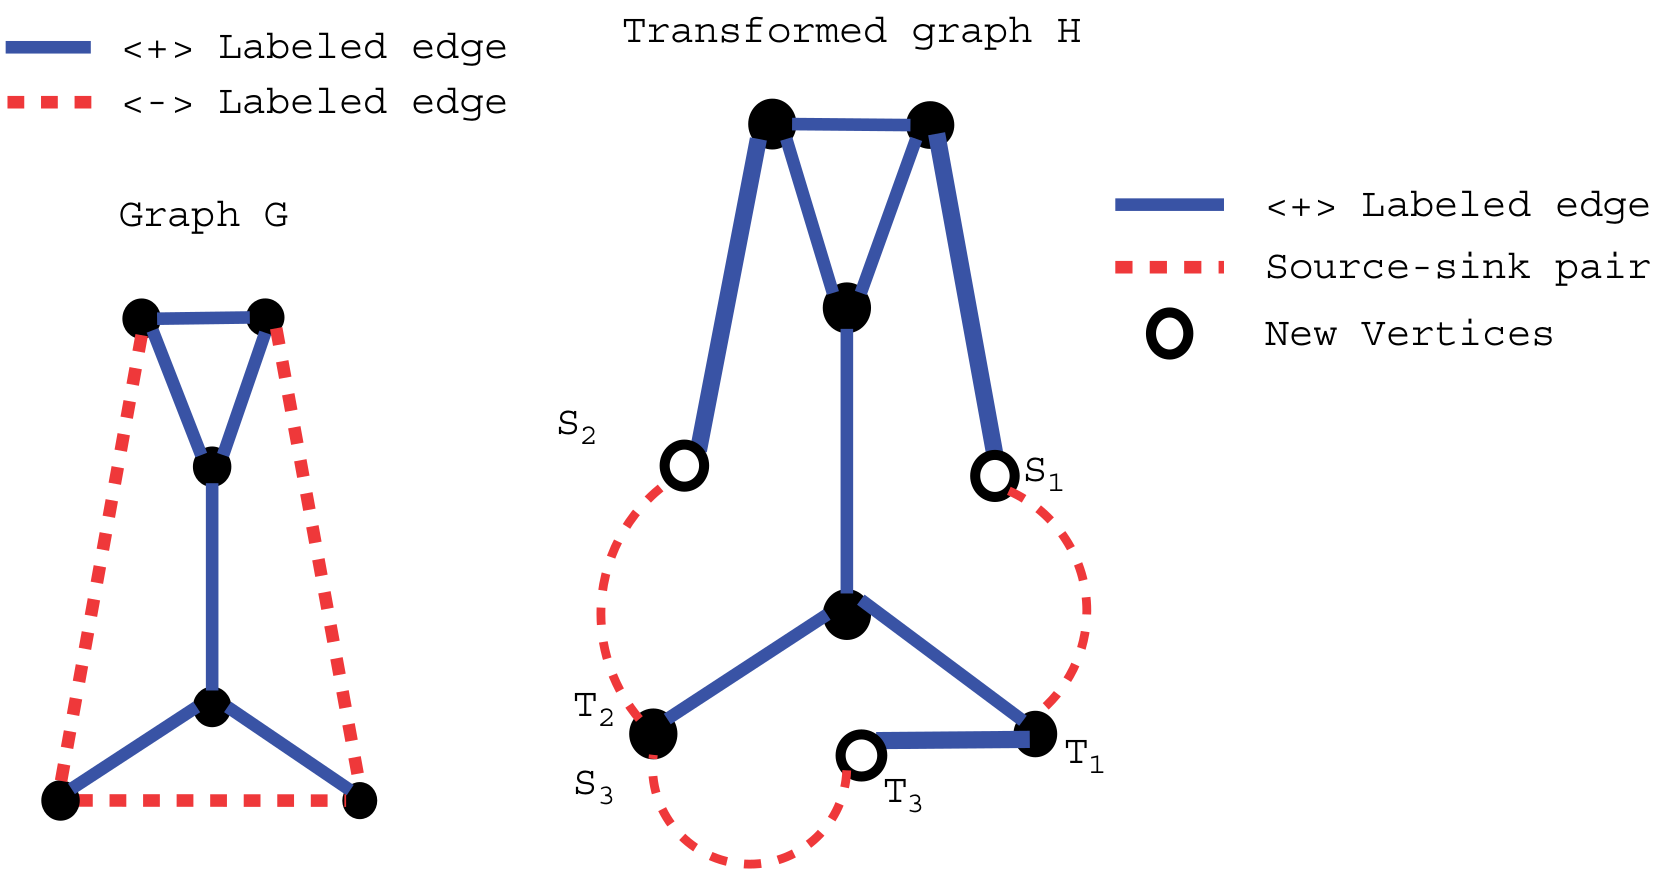
\includegraphics[width=0.8\linewidth]{assets/raw/cc_to_mmc.png}
   \caption{The transformation from \pcc{} on $G$ to \mmc{} on $H$ (temporarily reproduced from
   \autocite{Demaine2006}) \label{fig:cc_mmc}}
\end{figure}

\url{http://fpt.wikidot.com/fpt-races} and
\url{http://fpt.wikidot.com/complexity-status-of-edge-modification-problems} for parameterized
papers on \mmc{} and \textsc{Cluster Editing}.


Whereas clustering objective functions are \NPh{} to optimize, we expect that meaningful instances
in which we are interested have additional structure which allows for guaranteed polynomial time
algorithms, see for instance \autocite{clusteringFeasibility15} for a critical overview of some
proposed such notions of structure. Informally, a general idea is that the clustering should not
change (or at least very little) if the data are slightly perturbed. For instance, a weighted graph
is \emph{$\alpha$-stable} (with $\alpha>1$) for some partition objective if its optimal partition
remains the same whenever every weight $w_i$ is multiplied by a factor $c_i$ between $1$ and
$\alpha$. Finally, we say that an algorithm is \emph{robust} if, given an instance $\mathcal{I}$ and
in polynomial time, it: returns the optimal solution of $\mathcal{I}$ if $\mathcal{I}$ is
$\alpha$-stable; and if $\mathcal{I}$ is not $\alpha$-stable, either returns the optimal solution of
$\mathcal{I}$ or reports that $\mathcal{I}$ is not $\alpha$-stable. This is a handy property, as in
general, we cannot check the stability of an instance in practice as we do not know the optimal
solution hence we cannot tell whether it changes or not under perturbations.

\Textcite{StableCC17} provide a robust algorithm for $2-\nicefrac{2}{k}$-stable instance of
$k$-\textsc{Minimum Multiway Cut}, which therefore is not really useful in our case because I confused
multiway cut and multicut. To be fair, it seems I'm not the only one, \href{http://pages.cs.wisc.edu/~shuchi/papers/multicut-hardness-full.pdf}{on the hardness of
   approximating multicut}
   \enquote{multicut is known to be APX-hard
      (\href{https://pdfs.semanticscholar.org/1cf6/4c2bdd4f1c384a55910606a64c8d831a96ba.pdf}%
   {Dahlhaus et al. 1994}).} by that 1994 paper define the multiway cut problem, see
   \autoref{fig:cc_multiwhat}. \Textcite[Theorem 24]{Bansal2004} show that we can go from
   \textsc{Minimum Multiway Cut} to \pcc{} but I doubt about the other direction, mostly because
   \textsc{Minimum Multiway Cut} can actually be approximated with factor smaller than $1.3$.
   see \url{http://www.nowozin.net/sebastian/papers/nowozin2009lpstability.pdf} about LP multicut
   stability.
\begin{figure}[htpb]
   \centering
   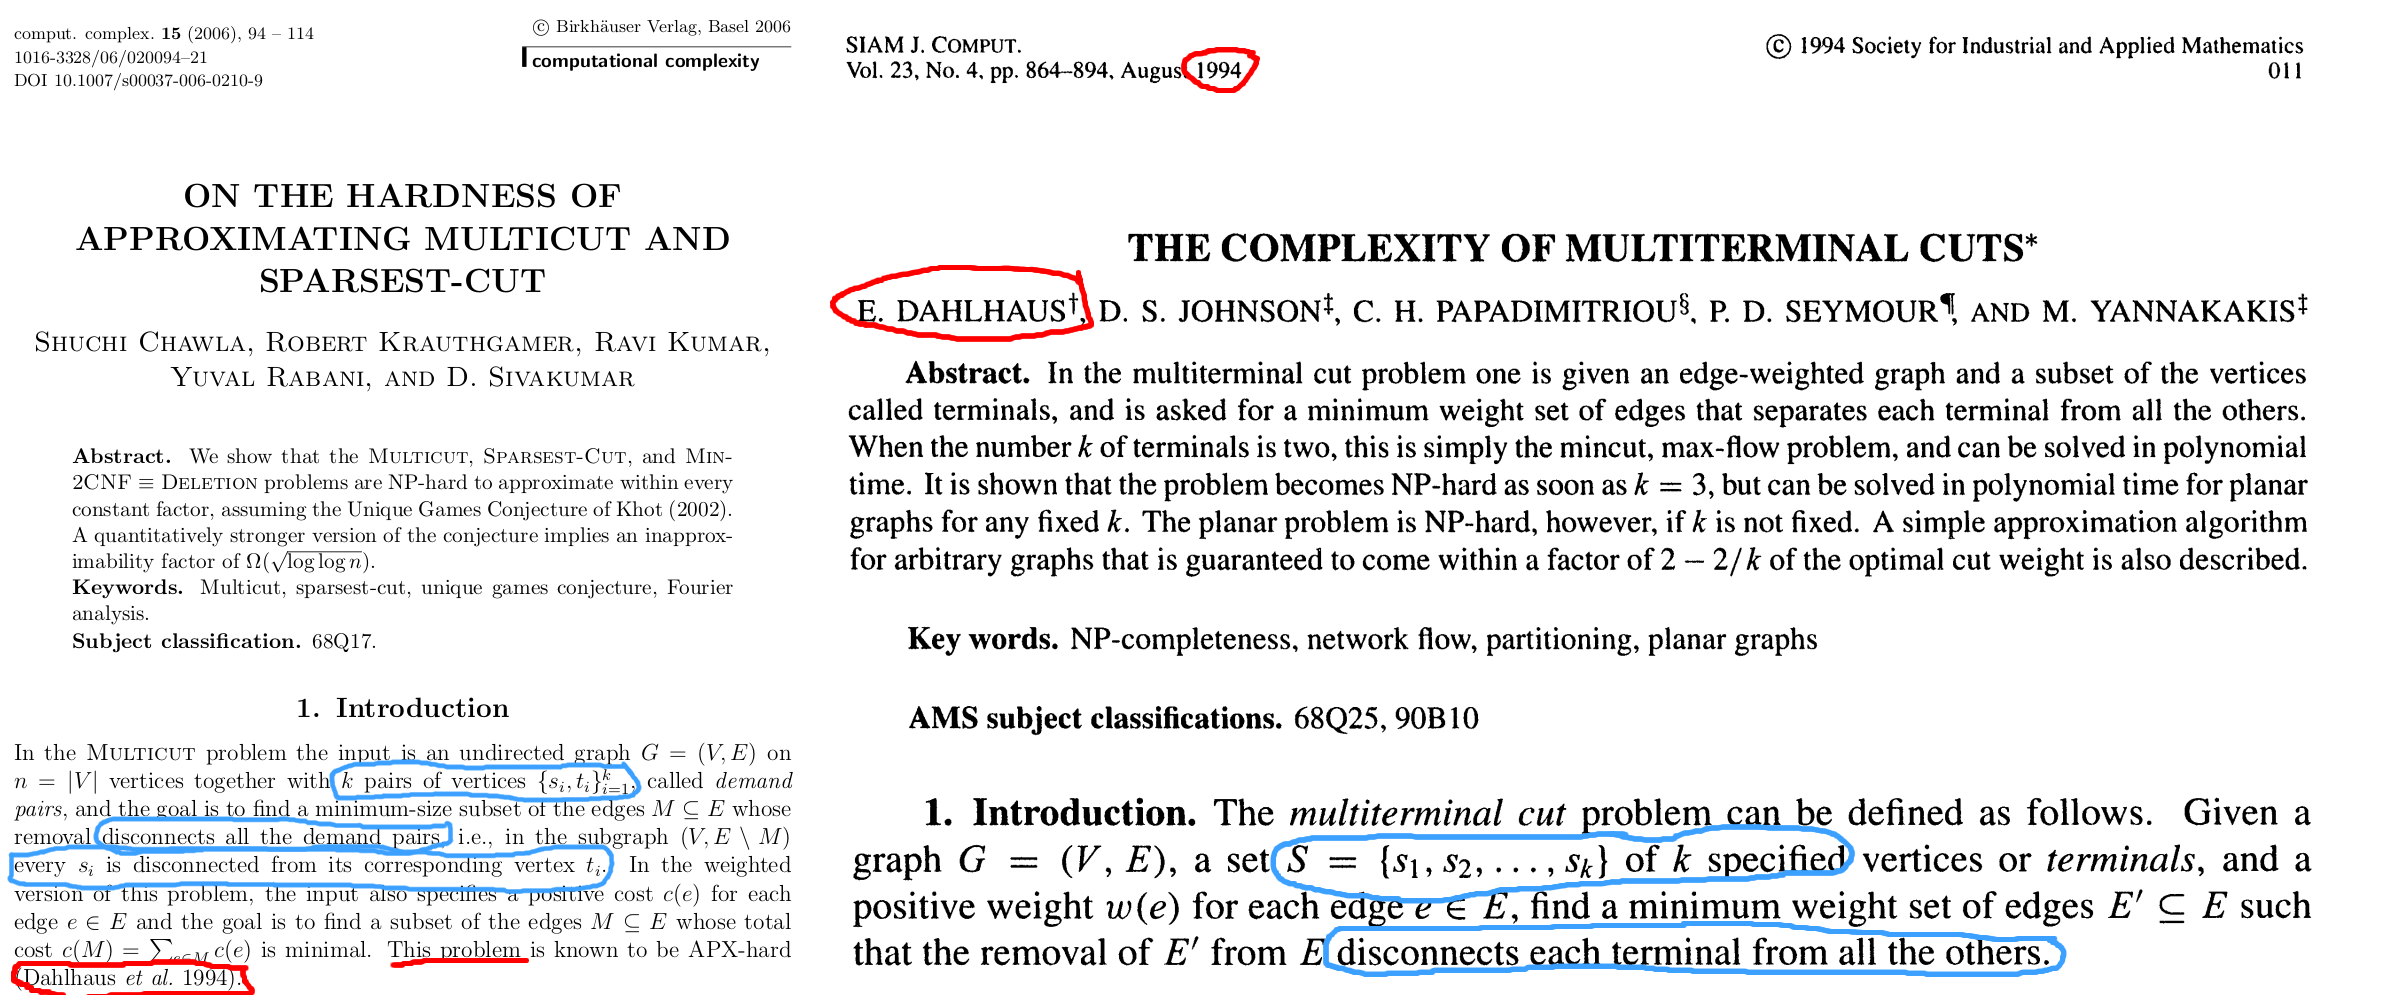
\includegraphics[width=0.9\linewidth]{assets/raw/multicut_vs_multiway.png}
   \caption{Confusing statement} \label{fig:cc_multiwhat}
\end{figure}


% \enquote{We prove that if the Unique Games Conjecture of Khot (2002) is true, then for every constant L > 0
% it is NP-hard to approximate Multicut within factor L. If a quantitatively stronger version of the
% conjecture is true, then Multicut is NP-hard to approximate within a factor of $\Omega(\sqrt{\log
% \log n})$.}

% It's probably limited because LP with a lot of constraints do not scale that well (someone claimed
% $O(n^{4.5})$)

% SDP Gaps and UGC Hardness for Multiway Cut, 0-Extension and Metric Labelling,
% On the Unique Games Conjecture: Subhash Khot
% under the UGC, one cannot get better than $O(\log n)$ approximation using LP or SDP relaxation.

